\subsection{Automating tactic exploration in the
background}\label{peacoq-design-automation}

In order to tackle our third identified challenge, that is, helping the user
discover what actions they may take in a given context, we experimented with an
automation technique.  The technique itself is simple: while the user is not
actively entering tactics, we can, in the background, generate and evaluate the
results of a large body of tactics.  We can then estimate which of those tactics
seems relevant to the users and choose how to display them to the user.

The difficulty lies in the details, in particular, we must address the following
problems:

\begin{itemize}

  \item what tactics to try,

  \item which results are relevant,

  \item and how to display those results we deem relevant.

\end{itemize}

We will cover those in order, describing the set of options available.  In our
evaluation, we will highlight which choices we made.

\subsubsection{What tactics to try?}

Because \Coq{} admits \Gallina{} terms as arguments to some \Ltac{} tactics,
there is effectively an infinite number of tactics that can be performed at any
step.  Even ignoring those, many tactics take terms in the environment as
arguments, and the standard library already introduces more than a thousand
terms in the ambient environment.  This makes it clear that an exhaustive search
is not likely.  A couple criteria will help us discern what tactics are worth trying.

First, we can differentiate tactics called \define{terminators} from the ones
that are not.  A terminator is a tactic whose success terminates the current
obligation.  Terminators come in different ways, from very simple ones that find
a proof or a contradiction in the immediate context, to solvers for a given
theory.  For instance, the \coqinline{assumption} tactic is a terminator that
simply looks for an assumption in the current context whose type equates to the
current goal (up to some notion of equality), while the \coqinline{omega} tactic
is a \define{complete} solver for \define{Presburger arithmetic}.  There are
only two outcomes out of the execution of a terminator: either the proof is
found and the tactic succeeds and finishes the current obligation, or its
execution fails.

On the other hand, non-terminator tactics can succeed either by finishing the
current obligation, or by modifying it in any way, or even not doing anything.
They can also lead to the creation of multiple obligations.  For instance, the
\coqinline{split} tactic succeeds on goals that contain a top-level
\define{conjunction}, possibly under a $\Pi$-telescope: it introduces all the
binders in the telescope, and yields two obligations, one for each conjunct.

It is best to test inexpensive terminators first, since a success would mean we
need not look further.  On the other hand, some terminators can effectively
diverge, either by taking an unreasonable amount of time, or by using an
increasingly larger amount of resources, eventually throttling.  In general, we
will need to account for such slowdowns for all tactics with a timeout
mechanism, as we don't want the automation machinery to have a negative
performance impact for our users.

A second important aspect to consider is what arguments to pass to tactics that
require them.  The families of \coqinline{apply} and \coqinline{rewrite}
tactics, for instance, all take as input one term to work with, and, for some, a
second term indicating where to perform the work.  Those terms can either be
variables that are local to the current proof context, or any variable that is
in scope from this file or imported files.  The latter set tends to be between
one and two orders of magnitude larger than the former.  Therefore, while it is
reasonable, but expensive, to try all the proof-local variables, it would be
very expensive to try all identifiers in scope!

\subsubsection{Which results are relevant?}

While we could display all the successful tactics and their outcome to the user,
the amount of information would, in most cases, be overwhelming.  In order for the suggestions to ever be useful, some triage is necessary.

After putting failing tactics out of the picture, one of our first remark is
that many tactics produce the exact same obligations.  Here, one might want to distinguish two close categories:

\begin{itemize}

  \item Two tactics may produce the exact same partial proof term, yielding
equal proof obligations.  This is obviously the case when the two tactics are
aliases of each other, but it can also happen when the two tactics take the same
simple logical step.  Let us refer to those as \define{proof-term equivalent
executions}.

  \item Two tactics may produce the exact same proof obligations (same goals
with same contexts), but build different proof terms.  This could be a concern,
when the terms being built have significant computational differences,
especially in settings where proofs are relevant.  Let us refer to those as
\define{proof-context equivalent executions}.

\end{itemize}

Ideally, we would like to factor out proof-term equivalent executions.  The user
might still care about what tactic is used.  For instance, wherever the
\coqinline{assumption} tactic works, tactics like \coqinline{auto} or
\coqinline{intuition} should also work, but they might do additional work that
is unnecessary.  Similarly, if the assumption being used is called
\coqinline{H}, the tactic \coqinline{exact H} should also work, but it might be
less robust to changes, especially if the name \coqinline{H} was
automatically introduced by \Coq{}.

Finally, the set of tactics available in the \Coq{} proof assistant is not
static: the tactic language is extensible, and users frequently define both
general-purpose and domain-specific tactics.  These can be registered as hints
to the built-in automation mechanism, in which case tactics like
\coqinline{auto} will use them appropriately.  However, as far as we know, at
the current time, there is no built-in mechanism for discovering user-defined
tactics in scope.  An automation mechanism would most likely benefit from such
domain-specific knowledge of tactics to be used in a given proof.

\subsubsection{How to display the relevant results?}

Displaying the outcome of the automation also proves an interesting challenge.
For terminators, or non-terminators that end up solving the current proof
obligation, we can simply indicate to the user that they do.  Tactics that make
progress without solving the proof, however, must be somehow shown to the user
alongside their result.  In the simplest form, one could just present a list of
those tactics, and let the user try them and witness their result on their own.
This imposes quite a bit of cognitive load on the users, as they must visually
inspect one or several proof obligations, trying to understand what changed
between before and after the tactic execution.

In order to reduce that effort, we developed a visualization that lets a user
quickly inspect the changes made to a proof context by the execution of a
tactic.  The idea is to provide a diff-like visualization, where changes are
highlighted, and items of the proof context that have appeared, disappeared, or
moved around are visually indicated as such.

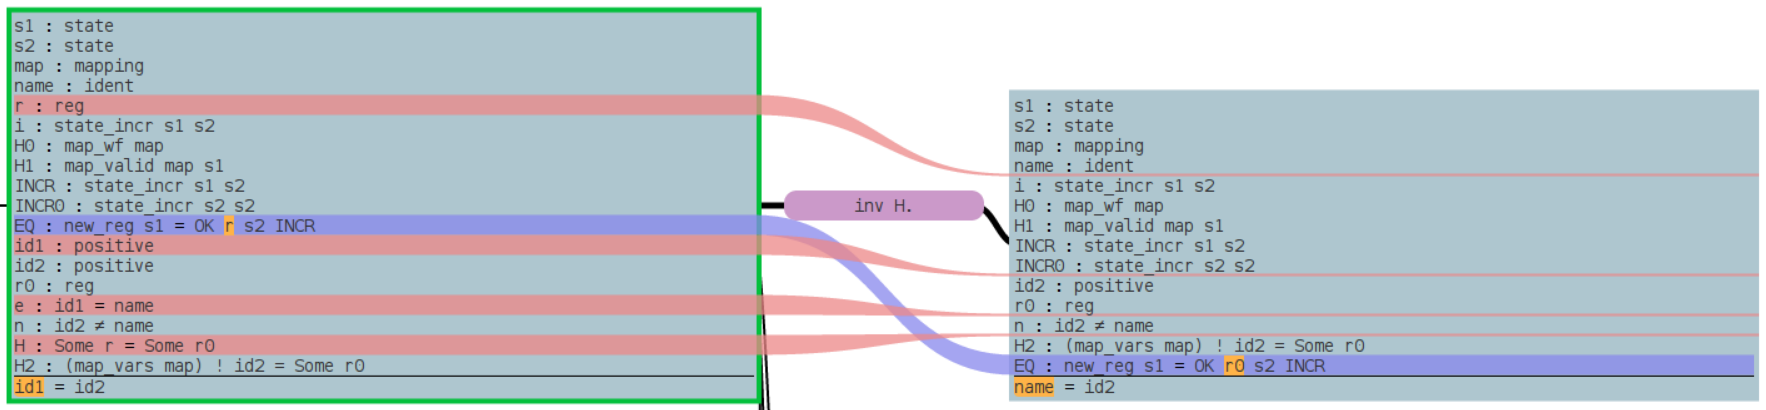
\includegraphics[width=\textwidth]{peacoq-diffs}{\parfillskip=0pt\par}

In our visualization, each proof obligation remaining after the execution of a
tactic can be visually aligned against the former proof obligation, and some
ribbons and highlights will appear to indicate changes made to the proof
obligation.  Hypotheses that have disappeared are indicated with a red,
shrinking ribbon, pointing to where they would have been.  Conversely,
hypotheses that have been introduced are indicated with a green ribbon, emerging
from where it has been introduced.  Finally, hypotheses that have undergone a
syntactic change or have moved around are indicated by a blue ribbon between
their old position and their now position, with additional syntactic
highlighting for the sub-terms of it that have changed.

Finally, while visual diffs allow the user to quickly inspect the outcome of a
given tactic, if there are too many tactics that make progress, going through
them all one by one can still require a lot of time and concentration.  Some
members of one of our studies indicated the need for grouping the results.  We
followed a static grouping strategy, where tactics were grouped together based
on similar intent: apply tactics, case analysis tactics, rewrite tactics,
terminators, etc.  This let users skip over entire classes of tactics that they
know are not what they are currently trying to achieve in the proof.
